\documentclass[12pt,a4paper]{article}

\usepackage{amsmath,amssymb,amsthm}
\usepackage{geometry}
\usepackage{microtype}
\usepackage{hyperref}
\usepackage{enumitem}
\usepackage{setspace}
\usepackage{booktabs}
\usepackage{graphicx}
\usepackage{xcolor}
\usepackage{tikz}
\usetikzlibrary{arrows.meta, decorations.pathmorphing, positioning, calc, shapes.geometric}

\geometry{margin=1.2in}
\setstretch{1.15}

\theoremstyle{plain}
\newtheorem{theorem}{Theorem}[section]
\newtheorem{proposition}[theorem]{Proposition}
\newtheorem{lemma}[theorem]{Lemma}
\newtheorem{corollary}[theorem]{Corollary}

\theoremstyle{definition}
\newtheorem{definition}[theorem]{Definition}
\newtheorem{example}[theorem]{Example}
\newtheorem{remark}[theorem]{Remark}

\hypersetup{
  colorlinks=true,
  linkcolor=black,
  citecolor=black,
  urlcolor=black
}

\title{\textbf{Geodesics of Attention}\\
\large Cinema, Gesture, and the Perceptual Manifold}

\author{Flyxion}

\date{}

\begin{document}

\maketitle
\thispagestyle{empty}

\begin{abstract}
We propose a unified geometric framework in which cinema, painting, drawing,
swipe-gesture input, and visual perception are instances of a single underlying
structure: directed motion through a structured spatial or perceptual field.
A film is modeled as a continuous path through a \emph{scenario manifold}
$\mathcal{S}$ whose coordinates encode camera pose, actor configuration,
lighting, and environmental state. The perceptual impact of that path is
determined not by its geometry in $\mathcal{S}$ but by its image under a
rendering-and-perception map $\Pi:\mathcal{S}\to\mathcal{P}$ into a
\emph{perceptual manifold} $\mathcal{P}$ whose coordinates are attentional
focus, revealed narrative information, occlusion structure, emotional intensity,
and compositional balance. We show that cinematographic naturalness corresponds
to approximate geodesic motion in $\mathcal{P}$ with respect to a metric tensor
derived from information geometry, and that narrative intent introduces a
potential function that forces the path toward perceptually salient states. This
variational principle unifies classical editing rules (the 180-degree rule, match
cuts, shot-reverse-shot) as geometric constraints on paths in $\mathcal{P}$.
We then extend the framework to cover painting strokes guided by image-gradient
fields, children's drawing as a sequential grammar of spatial occupation,
QWERTY swipe gestures as a trajectory language over a discrete keyboard manifold,
and eye saccades as perceptual sampling paths. Across all these cases, embodied
motion through a structured field generates symbolic or aesthetic meaning through
the same variational mechanism. The framework connects cinematography, game
engine simulation, information geometry, embodied cognition, and trajectory-based
generative models.
\end{abstract}

\newpage
\setcounter{page}{1}
\tableofcontents
\newpage

%% ------------------------------------------------------------------
\section{Introduction}
%% ------------------------------------------------------------------

Many cultural activities that seem superficially unrelated share a common deep
structure: they are all instances of directed motion through a structured spatial
or perceptual field, where meaning or aesthetic quality emerges from the shape
of that motion rather than from its endpoints alone. A filmmaker choosing a
camera angle, a painter laying down a brushstroke, a child completing a figure on
a page, a typist swiping a word, and a viewer's eye jumping between salient
features of a scene are all performing versions of the same cognitive and bodily
operation.

This paper proposes a unified mathematical framework for these activities. The
central object is a \emph{trajectory}: a continuous path $\gamma(t)$ through some
structured space, where the space is endowed with a geometry that determines
which paths are natural, smooth, or costly. We argue that the appropriate notion
of naturalness is always determined by a \emph{perceptual metric}---a metric
tensor on a manifold of experiential states---rather than by a purely physical or
symbolic metric.

The framework has five main components.

\begin{enumerate}[label=(\arabic*)]
\item \textbf{Scenario space $\mathcal{S}$}: the high-dimensional space of all
possible world states, including camera parameters, actor configurations,
lighting, and environment.

\item \textbf{Perceptual manifold $\mathcal{P}$}: the space of experiential
states as induced in a viewer, carrying a metric derived from information
geometry.

\item \textbf{Rendering-and-perception map $\Pi:\mathcal{S}\to\mathcal{P}$}:
the operator that converts scenario states into perceptual states.

\item \textbf{Geodesic principle}: cinematographic naturalness corresponds to
approximate geodesic motion in $\mathcal{P}$ subject to a narrative potential
function.

\item \textbf{Generality}: the same variational structure governs painting
strokes, drawing grammars, swipe gestures, and eye saccades.
\end{enumerate}

Modern film production already instantiates part of this structure. Virtual
production systems such as Unreal Engine represent a scene as a game state
$g = (C, A, L, E)$ whose components are camera pose, actor configurations,
lighting, and environment, and the camera path through that state space is
literally a trajectory. But a film recorded with a physical camera also
constitutes a path through a latent scenario space, whether or not that space is
ever explicitly simulated. The theoretical reinterpretation proposed here treats
this implicit structure as the object of analysis.

Section~\ref{sec:scenario} defines scenario space formally. Section~\ref{sec:perceptual}
introduces the perceptual manifold and its metric. Section~\ref{sec:geodesic}
states the geodesic principle and derives the variational equations.
Section~\ref{sec:editing} reinterprets classical editing conventions.
Section~\ref{sec:information} grounds the metric in information geometry.
Section~\ref{sec:painting} extends the framework to painting and visual gradients.
Section~\ref{sec:drawing} addresses children's drawing and the grammar of spatial
action. Section~\ref{sec:swipe} treats QWERTY swipe gestures as a trajectory
language. Section~\ref{sec:saccades} connects the framework to eye saccades and
embodied cognition. Section~\ref{sec:learning} discusses implications for
generative models. Section~\ref{sec:conclusion} concludes.

%% ------------------------------------------------------------------
\section{Scenario Space}
\label{sec:scenario}
%% ------------------------------------------------------------------

\begin{definition}[Scenario state]
A \emph{scenario state} is a tuple
\[
s = (C, A, L, E)
\]
where:
\begin{itemize}[nosep]
\item $C = (x,y,z,\theta,\phi,f) \in \mathbb{R}^6$ encodes camera position,
orientation angles, and focal length;
\item $A = (a_1,\dots,a_k)$ encodes the pose and animation state of each of $k$
actors in the scene;
\item $L$ encodes lighting configuration (source positions, intensities, color
temperatures);
\item $E$ encodes environmental parameters (weather, time of day, set geometry).
\end{itemize}
\end{definition}

The \emph{scenario manifold} $\mathcal{S}$ is the space of all valid scenario
states. For continuous physical parameters it is a smooth manifold; for
discrete categorical parameters (shot type, costume) it can be replaced by a
stratified space. We work in the smooth case throughout.

A \emph{film} in this framework is a smooth path
\[
\gamma: [0,T] \to \mathcal{S}.
\]
Each frame corresponds to a sample $s_t = \gamma(t)$. The observable image at
time $t$ is the output of a rendering operator:
\[
I_t = R(s_t),
\]
where $R:\mathcal{S}\to\mathcal{I}$ maps scenario states to images in some image
space $\mathcal{I}$. The observable film is therefore the sequence
$(I_t)_{t\in[0,T]}$, i.e., the image of the trajectory under $R$.

\begin{remark}
In a real-time game engine, $\mathcal{S}$ is the engine's world state and $R$
is the rendering pipeline. A film recorded on a physical set has the same
abstract structure, with $R$ replaced by the physical optics of the camera. The
theoretical framework applies to both.
\end{remark}

\begin{figure}[h]
\centering
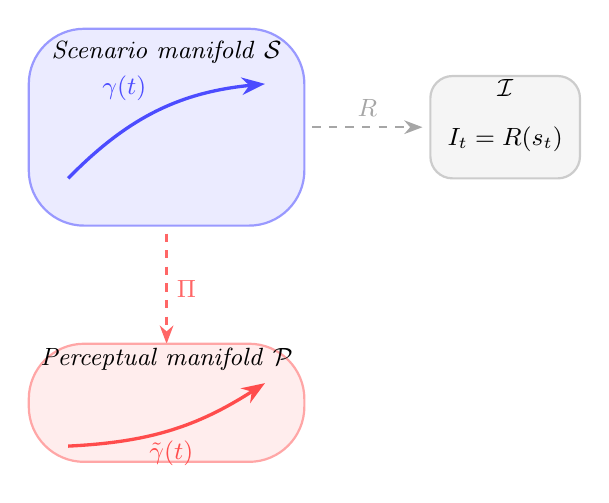
\begin{tikzpicture}[>=Stealth, thick, font=\small]
  % Scenario manifold blob
  \draw[fill=blue!8, draw=blue!40, rounded corners=20pt]
    (0,0) rectangle (3.5,2.5);
  \node at (1.75,2.2) {\textit{Scenario manifold} $\mathcal{S}$};
  % trajectory in S
  \draw[blue!70, very thick, ->, bend left=20]
    (0.5,0.6) to node[above left, pos=0.5]{$\gamma(t)$} (3.0,1.8);

  % arrow for R
  \draw[->, dashed, gray!70] (3.6,1.25) -- node[above]{$R$} (5.0,1.25);

  % Image space
  \draw[fill=gray!8, draw=gray!40, rounded corners=8pt]
    (5.1,0.6) rectangle (7.0,1.9);
  \node at (6.05,1.75) {$\mathcal{I}$};
  \node at (6.05,1.1) {$I_t = R(s_t)$};

  % Pi arrow downward
  \draw[->, dashed, red!60] (1.75,-0.1) -- node[right]{$\Pi$} (1.75,-1.5);

  % Perceptual manifold blob
  \draw[fill=red!7, draw=red!35, rounded corners=20pt]
    (0,-3) rectangle (3.5,-1.5);
  \node at (1.75,-1.7) {\textit{Perceptual manifold} $\mathcal{P}$};
  \draw[red!70, very thick, ->, bend right=15]
    (0.5,-2.8) to node[below, pos=0.5]{$\tilde\gamma(t)$} (3.0,-2.0);
\end{tikzpicture}
\caption{The scenario manifold $\mathcal{S}$, rendering map $R$, and
perceptual manifold $\mathcal{P}$. A film is a path $\gamma(t)$ in $\mathcal{S}$;
its aesthetic quality is determined by the induced path $\tilde\gamma(t)$ in
$\mathcal{P}$.}
\label{fig:manifolds}
\end{figure}

%% ------------------------------------------------------------------
\section{The Perceptual Manifold}
\label{sec:perceptual}
%% ------------------------------------------------------------------

The scenario manifold describes what the world \emph{is}; the perceptual
manifold describes what a viewer \emph{experiences}. A physically simple camera
move can feel disorienting, while a physically elaborate tracking shot can feel
effortless. The difference lies not in $\mathcal{S}$ but in $\mathcal{P}$.

\begin{definition}[Perceptual state]
A \emph{perceptual state} is a tuple
\[
p = (a, r, o, e, q) \in \mathcal{P}
\]
where:
\begin{itemize}[nosep]
\item $a \in [0,1]$ is attentional focus (concentration of viewer attention on a
primary subject);
\item $r \in [0,1]$ is revealed narrative information (cumulative proportion of
withheld story information disclosed);
\item $o \in [0,1]$ is occlusion coherence (stability of depth ordering and
figure-ground relations);
\item $e \in [0,1]$ is emotional intensity (arousal level induced by the scene);
\item $q \in [0,1]$ is compositional balance (degree of visual equilibrium in the
frame).
\end{itemize}
\end{definition}

The perceptual manifold $\mathcal{P}$ carries a Riemannian metric tensor
$g_{ij}(p)$ that measures the cognitive cost of moving between perceptual states.
The infinitesimal perceptual distance is
\[
ds^2 = \sum_{i,j=1}^{5} g_{ij}(p)\,dp^i\,dp^j.
\]

\begin{definition}[Rendering-and-perception map]
The \emph{rendering-and-perception map} is a smooth map
\[
\Pi: \mathcal{S} \to \mathcal{P}
\]
that assigns to each scenario state the perceptual state it induces in a
standard viewer. A film trajectory $\gamma(t)$ in $\mathcal{S}$ induces a
\emph{perceptual trajectory}
\[
\tilde\gamma(t) = \Pi(\gamma(t)) \in \mathcal{P}.
\]
\end{definition}

The derivative of $\Pi$ at a point $s \in \mathcal{S}$ is the Jacobian
$D\Pi_s: T_s\mathcal{S} \to T_{\Pi(s)}\mathcal{P}$.
The metric on $\mathcal{P}$ pulls back through $\Pi$ to a metric on $\mathcal{S}$:
\[
(D\Pi^* g)_s(u,v) = g_{\Pi(s)}(D\Pi_s\cdot u,\, D\Pi_s\cdot v),
\qquad u,v \in T_s\mathcal{S}.
\]
In this pullback metric, directions in $\mathcal{S}$ that induce large
perceptual change are far apart even if they are physically close.

%% ------------------------------------------------------------------
\section{Naturalness as a Geodesic Principle}
\label{sec:geodesic}
%% ------------------------------------------------------------------

\subsection{The action functional}

The perceptual length of a trajectory $\tilde\gamma$ over the interval $[0,T]$
is
\[
L[\tilde\gamma] = \int_0^T
\sqrt{g_{ij}(\tilde\gamma(t))\,\dot{\tilde\gamma}^i(t)\,\dot{\tilde\gamma}^j(t)}
\,dt.
\]
Minimizing $L$ is equivalent (up to reparametrization) to minimizing the
\emph{perceptual action}
\[
\mathcal{A}[\tilde\gamma]
= \frac{1}{2}\int_0^T
g_{ij}(\tilde\gamma(t))\,\dot{\tilde\gamma}^i(t)\,\dot{\tilde\gamma}^j(t)
\,dt.
\]

\begin{definition}[Cinematographically natural trajectory]
A perceptual trajectory $\tilde\gamma$ is \emph{cinematographically natural} if
it is a geodesic of $(\mathcal{P},g)$, i.e., if it satisfies the Euler-Lagrange
equations of $\mathcal{A}$.
\end{definition}

The Euler-Lagrange equations of $\mathcal{A}$ yield the \emph{geodesic equation}
\[
\ddot{\tilde\gamma}^k + \Gamma^k_{ij}\,\dot{\tilde\gamma}^i\,\dot{\tilde\gamma}^j = 0,
\]
where $\Gamma^k_{ij}$ are the Christoffel symbols of the metric $g$:
\[
\Gamma^k_{ij} = \frac{1}{2}g^{k\ell}
\!\left(
\partial_i g_{j\ell} + \partial_j g_{i\ell} - \partial_\ell g_{ij}
\right).
\]
The geodesic equation says that a natural camera path has no \emph{perceptual
acceleration}: it does not jerk the viewer's attention in unexpected directions.

\subsection{Narrative forcing}

A purely geodesic path in $\mathcal{P}$ does not capture the director's
intention to reveal information or guide attention toward specific story events.
We introduce a \emph{narrative potential} $V:\mathcal{P}\to\mathbb{R}$, where
low values of $V$ correspond to perceptually important or informationally rich
states. The forced trajectory satisfies
\[
\frac{D\dot{\tilde\gamma}}{dt} = -\nabla V(\tilde\gamma),
\]
where $D/dt$ denotes the covariant derivative along the path. This is the
geodesic equation with a forcing term: the director steers perception toward
narrative attractors (a face, a weapon, an emotionally decisive gesture) at the
cost of some perceptual smoothness.

\begin{definition}[Cinematic action with narrative potential]
The \emph{cinematic action} is
\[
\mathcal{J}[\tilde\gamma]
= \int_0^T
\!\left[
\frac{1}{2}\,g_{ij}(\tilde\gamma)\,\dot{\tilde\gamma}^i\,\dot{\tilde\gamma}^j
+ \lambda\,V(\tilde\gamma)
\right]dt,
\]
where $\lambda > 0$ is a weight balancing perceptual smoothness against
narrative urgency.
\end{definition}

\begin{proposition}
The Euler-Lagrange equations of $\mathcal{J}$ are
\[
\ddot{\tilde\gamma}^k
+ \Gamma^k_{ij}\,\dot{\tilde\gamma}^i\,\dot{\tilde\gamma}^j
+ \lambda\,g^{k\ell}\,\partial_\ell V(\tilde\gamma)
= 0.
\]
\end{proposition}

\begin{proof}
Standard variational calculus applied to the Lagrangian
$\mathcal{L}(p,\dot p) = \tfrac{1}{2}g_{ij}\dot p^i\dot p^j + \lambda V(p)$.
The first term gives the Christoffel-symbol term as in the pure geodesic case;
the second gives the gradient of $V$ raised by the inverse metric.
\end{proof}

\begin{remark}
The parameter $\lambda$ encodes directorial style. A director who prizes
compositional fluidity (Tarkovsky) operates at small $\lambda$; a director who
prioritizes narrative information density (Eisenstein) operates at large
$\lambda$.
\end{remark}

\begin{figure}[h]
\centering
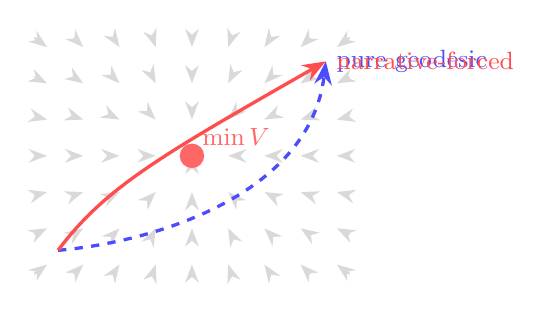
\begin{tikzpicture}[>=Stealth, thick, font=\small]
  % background field for V
  \foreach \x in {0,0.5,...,4}{
    \foreach \y in {0,0.5,...,3}{
      \pgfmathsetmacro{\len}{0.18}
      \pgfmathsetmacro{\dx}{-(\x-2.0)*0.08}
      \pgfmathsetmacro{\dy}{-(\y-1.5)*0.08}
      \draw[gray!30, ->] (\x,\y) -- ++(\dx,\dy);
    }
  }
  % attractor
  \filldraw[red!60] (2.0,1.5) circle (4pt) node[above right]{$\min V$};
  % geodesic path (no forcing)
  \draw[blue!70, dashed, very thick, ->]
    (0.3,0.3) .. controls (1.5,0.4) and (3.5,1.0) .. (3.7,2.7)
    node[right]{pure geodesic};
  % forced path
  \draw[red!70, very thick, ->]
    (0.3,0.3) .. controls (0.9,1.1) and (1.6,1.5) .. (3.7,2.7)
    node[right]{narrative-forced};
\end{tikzpicture}
\caption{Narrative forcing bends the geodesic toward the attractor $\min V$
(the narratively important perceptual state) at the cost of some smoothness.
The pure geodesic ignores narrative structure; the forced path balances
perceptual economy with directorial intent.}
\label{fig:forcing}
\end{figure}

%% ------------------------------------------------------------------
\section{Editing as Trajectory Transformation}
\label{sec:editing}
%% ------------------------------------------------------------------

Film editing introduces discontinuities or structured transformations in the
scenario trajectory $\gamma$. We show how classical editing operations correspond
to geometric operations on paths in $\mathcal{S}$ and $\mathcal{P}$.

\subsection{Cuts}

A \emph{hard cut} at time $t_0$ is a jump discontinuity:
\[
\gamma(t_0^-) \neq \gamma(t_0^+).
\]
In $\mathcal{P}$, the corresponding perceptual jump $\tilde\gamma(t_0^-)
\neq \tilde\gamma(t_0^+)$ has a perceptual cost proportional to
$d_\mathcal{P}(\tilde\gamma(t_0^-), \tilde\gamma(t_0^+))$.

A cut is \emph{invisible} when the perceptual distance across the cut is small,
i.e., when the cut preserves attentional focus, occlusion coherence, and
compositional balance. This is the geometric content of the classical principle
of \emph{continuity editing}.

\subsection{Dissolves and wipes}

A \emph{dissolve} interpolates between two scenario states:
\[
I_t = (1-\alpha(t))\,R(\gamma_1(t)) + \alpha(t)\,R(\gamma_2(t)),
\quad \alpha:[0,1]\to[0,1].
\]
In $\mathcal{P}$, this corresponds to a blended perceptual path. The dissolve
is perceptually smooth when the two source paths $\Pi(\gamma_1)$ and
$\Pi(\gamma_2)$ are close in $\mathcal{P}$.

\subsection{Montage}

A \emph{montage sequence} is a piecewise trajectory
$\gamma = (\gamma_1,\gamma_2,\dots,\gamma_k)$
with jump discontinuities at the joints. In contrast to continuity editing,
montage deliberately creates large perceptual jumps. The Eisenstein principle
is that conceptually or emotionally significant jumps along certain coordinates
of $\mathcal{P}$ (especially $e$ and $r$) can generate meaning even at high
perceptual cost.

\subsection{The 180-degree rule}

The 180-degree rule constrains the camera trajectory to one side of an
imaginary line connecting the principal actors. In scenario-space terms, if
actors define an axis $\ell \subset \mathbb{R}^3$, the camera must satisfy
\[
C \in \mathcal{H}_+ = \{C : \langle n, \pi_\ell(C) \rangle > 0\}
\]
for a normal $n$ to $\ell$. Crossing this line corresponds to a large jump in
the occlusion coordinate $o$ of $\mathcal{P}$, because the left-right mapping
of actors is reversed. The 180-degree rule thus minimizes perceptual cost in
the $o$ coordinate; violating it forces a large excursion in $\mathcal{P}$.

\begin{proposition}
The 180-degree rule is the condition that the camera trajectory remains within a
single chart of $\mathcal{P}$ with respect to the occlusion coordinate $o$.
Crossing the line corresponds to a coordinate singularity in that chart.
\end{proposition}

\subsection{Match cuts and eyeline matches}

A \emph{match cut} transitions between two shots whose perceptual states are
closely aligned: similar attentional focus $a$, similar compositional balance
$q$, and continuous motion energy in $e$. Formally, a match cut at time $t_0$
satisfies
\[
\|\tilde\gamma_1(t_0^-) - \tilde\gamma_2(t_0^+)\|_\mathcal{P} < \varepsilon
\]
for small $\varepsilon$. The match cut is the editorial operation that minimizes
the perceptual distance across a cut.

An \emph{eyeline match} aligns the attentional direction of one shot with the
implied object of attention in the next, preserving continuity in the $a$
coordinate of $\mathcal{P}$.

%% ------------------------------------------------------------------
\section{Information Geometry of the Perceptual Metric}
\label{sec:information}
%% ------------------------------------------------------------------

\subsection{Viewer attention as a probability distribution}

We ground the metric $g$ on $\mathcal{P}$ in information geometry by modeling
the viewer's attentional state as a probability distribution over scene elements.

Let $\mathcal{X}$ be the set of salient objects in the frame (faces, hands,
weapons, etc.). The viewer's attentional state at time $t$ is a distribution
\[
P_t \in \Delta(\mathcal{X}),
\]
the probability simplex over $\mathcal{X}$. The \emph{attentional cost} of
moving from $P_t$ to $P_{t+dt}$ is measured by a divergence in this simplex.

\subsection{The Fisher-Rao metric}

When $P_t$ is parameterized by coordinates $\theta \in \Theta$, the
\emph{Fisher information metric} is
\[
g_{ij}^F(\theta)
= \mathbb{E}_{P(\cdot;\theta)}\!\left[
\frac{\partial \log P(x;\theta)}{\partial\theta^i}
\frac{\partial \log P(x;\theta)}{\partial\theta^j}
\right].
\]
This is the natural Riemannian metric on the statistical manifold
$\{P(\cdot;\theta):\theta\in\Theta\}$. Geodesics in this metric correspond to
paths of least inferential surprise: the viewer's belief about what is important
in the frame changes as smoothly as possible.

\begin{theorem}
The perceptual metric $g$ on $\mathcal{P}$ can be taken to be (or to dominate)
the Fisher-Rao metric on the manifold of attentional distributions. A camera
trajectory is perceptually smooth if and only if the induced path in
$\Delta(\mathcal{X})$ has bounded Fisher-Rao velocity.
\end{theorem}

\begin{proof}[Proof sketch]
The attentional coordinate $a$ of $\mathcal{P}$ determines the centroid of the
distribution $P_t$ over salient objects. The other coordinates $(r,o,e,q)$
introduce additional geometric structure. Since the Fisher-Rao metric is the
unique (up to scale) Riemannian metric on $\Delta(\mathcal{X})$ that is
invariant under sufficient statistics \cite{chentsov1982}, bounding its velocity
bounds the rate of change of all attentional quantities. The claim follows from
the smoothness of the parameterization by $(a,r,o,e,q)$.
\end{proof}

\subsection{Continuity editing as minimal attentional transport}

Continuity editing works by keeping the attentional transport cost low across
cuts. Formally, a cut at time $t_0$ transitions from distribution $P^-$ to
distribution $P^+$. The cost is
\[
W_2(P^-, P^+) = \inf_{\pi \in \Pi(P^-,P^+)}
\left(\int d(x,y)^2\,d\pi(x,y)\right)^{1/2},
\]
where $W_2$ is the Wasserstein-2 distance and the infimum is over couplings
$\pi$. A cut is invisible when $W_2(P^-,P^+)$ is small: the viewer's attention
can be transported cheaply from the pre-cut to the post-cut distribution.

This gives a precise measure-theoretic account of why continuity editing
works: it minimizes the optimal transport cost of viewer attention across
shot boundaries.

%% ------------------------------------------------------------------
\section{Painting as Gradient-Field Integration}
\label{sec:painting}
%% ------------------------------------------------------------------

\subsection{The image as a scalar field}

A painting-in-progress at time $t$ can be represented as a scalar field
$B_t:\Omega\to\mathbb{R}$, where $\Omega\subset\mathbb{R}^2$ is the canvas and
$B_t(x,y)$ encodes luminance or tonal value. A brushstroke is a trajectory
\[
\gamma_{paint}:[0,\tau]\to\Omega
\]
that updates the canvas field:
\[
B_{t+dt}(x,y) = B_t(x,y) + K(x-\gamma_x(t),\,y-\gamma_y(t)),
\]
where $K$ is the brush footprint kernel. Painting is therefore the process of
\emph{writing trajectories into a field}.

\subsection{The gradient field and isophotes}

The structural information in the image is encoded in the gradient field
\[
\nabla B = \left(\frac{\partial B}{\partial x},\frac{\partial B}{\partial y}\right).
\]
In computer vision this is approximated by Sobel filters:
\[
G_x = S_x * B,\qquad G_y = S_y * B,\qquad |\nabla B| = \sqrt{G_x^2+G_y^2}.
\]
Painters often orient strokes along the \emph{isophote} direction, tangent to
level curves of $B$:
\[
T = (-B_y,\, B_x).
\]
A stroke guided by this field satisfies
\[
\frac{d\gamma_{paint}}{dt} = \alpha\,T(\gamma_{paint}(t)) + \beta\,\nabla B(\gamma_{paint}(t)),
\]
where $\alpha$ controls how much the stroke follows the form contour and $\beta$
controls how much it follows the tonal gradient.

\subsection{Structure tensor and stroke direction}

The local orientation of image structure can be summarized by the
\emph{structure tensor}
\[
J = \begin{pmatrix} B_x^2 & B_x B_y \\ B_x B_y & B_y^2 \end{pmatrix}.
\]
The dominant eigenvector of $J$ gives the preferred local orientation of edges
and forms. A painter's stroke tends to follow this direction because it preserves
the perceived structure of the surface.

\begin{proposition}
A painter who aligns brushstrokes with the dominant eigenvector field of $J$
is integrating a vector field derived from the tonal gradient of the scene.
Each stroke is a geodesic segment in the metric induced by $J$ on $\Omega$.
\end{proposition}

\subsection{Comparison with cinematography}

The analogy with the cinematic case is precise. In both systems:
\begin{itemize}[nosep]
\item there is a trajectory $\gamma(t)$ through a structured space;
\item there is a field (tonal gradient in $\Omega$; perceptual metric on
$\mathcal{P}$) that determines which paths are natural;
\item naturalness corresponds to geodesic or near-geodesic motion in that field.
\end{itemize}
The difference is that in painting the trajectory modifies the field it moves
through (the canvas changes with each stroke), while in cinematography the
trajectory merely samples a pre-existing scenario manifold.

%% ------------------------------------------------------------------
\section{Drawing as a Sequential Grammar of Spatial Action}
\label{sec:drawing}
%% ------------------------------------------------------------------

\subsection{Goodnow's grammar of action}

Jacqueline Goodnow's empirical studies of children's drawing demonstrate that
drawings are not arbitrary marks but records of structured action sequences
\cite{goodnow1977}. Children follow systematic strategies for initiating
figures, attaching new elements, and expanding outward. Goodnow called these
strategies a \emph{grammar of action}: a set of procedural rules governing how
actions combine to produce spatial structures.

In the framework developed here, a drawing is a sequence of trajectories
\[
\gamma_1, \gamma_2, \dots, \gamma_n
\]
each depositing a stroke on the canvas field $B$. The grammar of action governs
the conditional distribution of $\gamma_{k+1}$ given the current canvas state
$B_{t_k}$ after the $k$-th stroke.

Formally, let the drawing process be an iterative mapping
\[
B_{t+1} = F(B_t, a_t),
\]
where $a_t$ is the stroke action chosen at step $t$ according to the grammar.
Goodnow's finding that children follow systematic attachment and expansion rules
means that $F$ is not arbitrary: new strokes are placed near existing structures,
extend boundaries, or occupy regions that preserve compositional balance.

\subsection{Developmental stages as metric learning}

Goodnow's developmental progression from simple attachment rules in young
children to symmetric, hierarchically organized compositions in older children
can be interpreted as the progressive acquisition of a more refined metric on
the space of compositional states. Young children use a coarse metric in which
proximity is the dominant criterion. Older children use a metric that also weighs
symmetry, distribution, and relational coherence.

\subsection{Kellogg's primitive trajectories}

Rhoda Kellogg's catalog of recurring scribble forms in children's early drawing
provides a vocabulary of trajectory primitives \cite{kellogg1969}:
\begin{itemize}[nosep]
\item loops (near-circular closed paths);
\item spirals (outwardly expanding loops);
\item zigzags (alternating diagonal segments);
\item arches (smooth convex arcs);
\item radiating lines (spokes from a central point).
\end{itemize}
These primitives correspond to the simplest geodesic shapes available in the
plane: constant-curvature curves (circles, arches), piecewise-linear paths
(zigzags), and self-similar expanding paths (spirals). Kellogg's observation
that these forms appear cross-culturally before representational drawing
develops supports the claim that the trajectory grammar is prior to, and
independent of, semantic representation.

%% ------------------------------------------------------------------
\section{QWERTY Swipe as a Trajectory Language}
\label{sec:swipe}
%% ------------------------------------------------------------------

\subsection{The keyboard as an embedded graph}

Let $K = (V,E)$ be the QWERTY keyboard graph, where each key is a vertex
$v \in V$ and edges connect neighboring keys. The graph is embedded in the
plane by the coordinate map
\[
\phi: V \to \mathbb{R}^2,
\]
which assigns each key its physical center position. This embedding makes $K$ a
\emph{finite metric space} in the induced Euclidean metric.

\begin{definition}[Swipe word trajectory]
For a word $w = w_1 w_2 \cdots w_n$ over the keyboard alphabet $\Sigma = V$,
the \emph{swipe trajectory} is the piecewise-linear path
\[
P(w) = (\phi(w_1), \phi(w_2), \dots, \phi(w_n)) \subset \mathbb{R}^2.
\]
\end{definition}

\begin{theorem}[Trajectory encoding]
The map $P:\Sigma^*\to\mathcal{T}$ from words to piecewise-linear trajectories
is a compositional encoding of the free monoid $(\Sigma^*,\cdot)$ into a space
$\mathcal{T}$ of planar paths. Hence QWERTY swipe induces a formal language for
representing trajectory classes.
\end{theorem}

\begin{proof}
The concatenation $w = uv$ of two words maps to the path concatenation
$P(w) = P(u) \cdot P(v)$ (joined at the endpoint of $P(u)$). This is the
monoid homomorphism property. The map is nontrivial because distinct words
generically produce distinct polygonal chains. Hence $P$ is a nontrivial
homomorphism from $(\Sigma^*,\cdot)$ into $(\mathcal{T}, \cdot)$.
\end{proof}

\subsection{Geometric invariants of words}

Each word $w$ has a geometric signature under $P$:
\begin{align*}
L(w) &= \sum_{i=1}^{n-1}\|\phi(w_{i+1})-\phi(w_i)\|
  &\text{(path length)},\\
C(w) &= \sum_{i=2}^{n-1}|\theta_i|
  &\text{(turn complexity)},\\
X(w) &= \text{(number of self-intersections of }P(w)\text{)},\\
\kappa_{\mathrm{close}}(w) &= 1 - \frac{\|\phi(w_n)-\phi(w_1)\|}{L(w)}
  &\text{(closure index)}.
\end{align*}

\begin{definition}[Trajectory equivalence]
Two words $w, u \in \Sigma^*$ are \emph{trajectory-equivalent} if their
normalized swipe paths are within $\varepsilon$ in Fréchet distance:
\[
w \sim u \iff d_F(\widetilde P(w), \widetilde P(u)) < \varepsilon,
\]
where $\widetilde P$ denotes the arc-length-normalized version of $P$.
\end{definition}

Trajectory equivalence classes define a \emph{gesture morphology}: families of
words that share a common kinematic shape regardless of their semantic or
phonological properties.

\subsection{Examples: geometric taxonomy of words}

Informal inspection of QWERTY swipe trajectories reveals that common words fall
into recognizable shape families:

\begin{center}
\begin{tabular}{llll}
\toprule
\textbf{Shape class} & \textbf{Example word} & \textbf{Dominant feature} \\
\midrule
Loop / circle   & \textit{tent}   & high closure index $\kappa_{\mathrm{close}}$ \\
Rectilinear     & \textit{route}  & few turn directions, dominant orthogonal phases \\
Braided / pretzel & \textit{magic} & $X(w) \geq 1$ (self-intersection) \\
Arch            & \textit{con}    & smooth convex arc, $C(w)$ small \\
Hook            & \textit{do}     & short path, large single turn \\
Ribbon sweep    & \textit{all}    & large $L(w)$, small $C(w)$, near-linear \\
Spiral          & \textit{crying} & increasing radius, monotone turning \\
Zigzag          & \textit{Zeno}   & alternating diagonal segments \\
\bottomrule
\end{tabular}
\end{center}

\begin{corollary}
Any lexicon $\mathcal{L}\subset\Sigma^*$ inherits a \emph{trajectory semantics}
via $P$, making the lexicon simultaneously a symbolic language and a geometric
codebook. The natural language vocabulary is a proper submanifold of the full
swipe trajectory space.
\end{corollary}

\subsection{The keyboard as a discrete canvas}

The keyboard can be interpreted as a discretized version of the painter's canvas:
instead of depositing pigment continuously, the gesture snaps to discrete letter
centers. Swipe typing is therefore a quantized painting system in which the
interpretation of a trajectory produces symbols rather than pigment.

The dual reading of a swipe word is:
\[
w \mapsto (\text{semantic meaning},\, \text{gesture class}).
\]
Natural language words function as compressed geometric operators: each word
is simultaneously semantic and kinematic.

%% ------------------------------------------------------------------
\section{Eye Saccades and Embodied Perception}
\label{sec:saccades}
%% ------------------------------------------------------------------

\subsection{Saccadic paths as perceptual trajectories}

Visual perception does not occur through smooth continuous scanning. The eye
moves through sequences of rapid fixation jumps called \emph{saccades}. If
fixation points are $p_1, p_2, \dots, p_n \in \mathcal{I}$, the visual scan
path is a trajectory
\[
\gamma_{eye}(t)
\]
through the image plane $\mathcal{I}$.

Saccades are not random: they are guided by a \emph{saliency field}
$\sigma:\mathcal{I}\to\mathbb{R}_{\geq 0}$, where high saliency corresponds to
edges, faces, motion, and high-contrast regions. The saccade trajectory
approximately maximizes accumulated saliency subject to a motor cost for large
eye movements. This is a constrained optimization structurally identical to the
variational principle of Section~\ref{sec:geodesic}.

\subsection{Three trajectory systems in the perceptual-motor loop}

We now see that three trajectory systems operate jointly in visual culture:

\begin{center}
\begin{tabular}{lll}
\toprule
\textbf{System} & \textbf{Body part} & \textbf{Output} \\
\midrule
Eye saccades   & Ocular muscles  & Perceptual sampling \\
Brush strokes  & Arm and hand    & Image construction \\
Swipe gestures & Finger          & Symbol generation \\
\midrule
\multicolumn{3}{l}{All three: trajectory $\gamma(t)$ through a structured field} \\
\bottomrule
\end{tabular}
\end{center}

The hand trajectory of the painter tends to follow the same image features that
the eye's saccades follow (edges, contours, saliency peaks). This is because both
are guided by the same gradient field of the image: the painter is externalizing
the scan path of the visual system as a stroke.

\subsection{Mimetic hypothesis and motor simulation}

Arnie Cox's \emph{mimetic hypothesis} holds that music perception recruits
internal motor representations: listeners simulate the bodily actions that could
produce the perceived sounds \cite{cox2016}. The perceptual trajectory in that
case moves through \emph{motor activation space} rather than image space.

Central pattern generators (CPGs) provide a neural substrate for such
simulations. A CPG chain produces rhythmic sequences of motor states:
\[
m_{t+1} = F(m_t),
\]
a trajectory through motor state space that can be driven by auditory input.
Baddeley's phonological loop is a cyclic CPG:
\[
a_1 \to a_2 \to \cdots \to a_n \to a_1,
\]
maintaining verbal information through repeated traversal of an articulatory
trajectory.

The unified claim is therefore:

\begin{quote}
\emph{Perception and expression across modalities share a common structure:
they are trajectories through structured fields, whether those fields are
spatial gradients on a canvas, geometric lattices on a keyboard, saliency maps
in an image, or motor activation manifolds in the nervous system.}
\end{quote}

%% ------------------------------------------------------------------
\section{Developmental Arc: From Object Grammar to Gradient Field}
\label{sec:developmental}
%% ------------------------------------------------------------------

Artistic development can be interpreted as a shift in the representational model
underlying trajectory production. This shift moves through three conceptual
layers.

\textbf{Stage 1: Object-oriented.} The page is treated as a set of discrete
entities. A drawing is an object graph $G = (R,E)$ where regions $R_i$
correspond to symbolic shapes (circle for head, lines for limbs) and edges $E$
encode attachment or containment. Strokes follow object boundaries. This is the
stage described by Goodnow's grammar of action in early childhood.

\textbf{Stage 2: Field-based.} The page becomes a tonal field $I(x,y)$. Strokes
follow the gradient and isophote structure of the field rather than symbolic
object boundaries. The artist observes continuous phenomena (shadow, reflection,
graduated tone) and reconstructs them as trajectories through the gradient field.

\textbf{Stage 3: Radiance model.} The experienced artist understands the image
as the projection of a physical light-transport process. Strokes implicitly
reconstruct the radiance field, solving the inverse problem:
\[
L_o(x,\omega) = L_e(x,\omega)
+ \int_\Omega f_r(x,\omega',\omega)\,L_i(x,\omega')\,(\omega'\cdot n)\,d\omega'.
\]
The artist does not compute this integral, but has internalized how light behaves
and places strokes that reproduce its effects. In computer graphics this is the
rendering equation; in artistic practice it is the implicit model that separates
expert from novice draughtsmen.

This three-stage arc corresponds to a progression from a symbolic object metric
to an information-geometric field metric as the criterion for naturalness of
strokes.

%% ------------------------------------------------------------------
\section{Learning Cinematic Trajectories}
\label{sec:learning}
%% ------------------------------------------------------------------

The variational framework suggests a natural approach to learning cinematic
style from observed films.

Given a corpus of films with associated perceptual state sequences
$\tilde\gamma_1, \tilde\gamma_2, \dots, \tilde\gamma_N$ (approximated through
automatic annotation of attention, composition, and narrative labels), one can
learn:
\begin{enumerate}[label=(\alph*)]
\item the metric $g_\theta$ on $\mathcal{P}$ by fitting a Riemannian metric
to minimize geodesic deviation of observed trajectories;
\item the potential $V_\phi$ by fitting the forced geodesic equation to
observed perceptual paths;
\item the rendering-and-perception map $\Pi_\psi$ by learning to predict
perceptual coordinates from scenario states.
\end{enumerate}

A generative cinematography system would then sample new scenario trajectories
$\gamma(t)$ that induce target perceptual trajectories $\tilde\gamma(t)$
minimizing $\mathcal{J}[\tilde\gamma]$ for a specified narrative potential.

\begin{remark}
This framework is compatible with diffusion-based video generation models, where
the denoising trajectory can be interpreted as navigation through scenario space.
Conditioning on a perceptual metric and narrative potential constrains the
generative trajectory to cinematographically natural paths.
\end{remark}

Applications include:
\begin{itemize}[nosep]
\item automatic cinematography for virtual production environments;
\item camera planning algorithms in game engines;
\item film style analysis and director fingerprinting;
\item trajectory-based video generation with aesthetic constraints;
\item gesture-driven interfaces for creative tools.
\end{itemize}

%% ------------------------------------------------------------------
\section{Conclusion}
\label{sec:conclusion}
%% ------------------------------------------------------------------

We have proposed a unified geometric framework in which diverse cultural
practices---cinema, painting, drawing, swipe-gesture input, and visual
perception---share a common mathematical structure: directed motion through a
structured field, where naturalness is determined by a variational principle on
a Riemannian manifold.

The central theoretical contribution is the \emph{geodesic principle of
cinematography}: natural camera movement approximates a geodesic in the
perceptual manifold $\mathcal{P}$, subject to forcing by a narrative potential
$V$. This principle unifies classical editing conventions (continuity, the
180-degree rule, match cuts, montage) as geometric constraints on paths in
$\mathcal{P}$, and grounds them in information geometry through the Fisher-Rao
metric on the manifold of viewer attentional distributions.

The same variational structure governs the painter's brush (guided by tonal
gradient fields), the child's drawing hand (constrained by a grammar of spatial
action), the typist's swiping finger (moving through a discrete keyboard
manifold), and the viewer's eye (jumping between salient image features).
Across all these modalities, meaning and aesthetic quality emerge from the shape
of motion through a structured field, not from the endpoint of that motion.

This framework has both theoretical and practical implications. Theoretically,
it provides a unifying vocabulary for disparate fields: cinematography, embodied
cognition, information geometry, art education, and human-computer interaction.
Practically, it suggests principled methods for learning and generating
cinematographically natural trajectories, designing gesture interfaces whose
vocabulary is geometrically coherent, and analyzing artistic style as a
characteristic signature in trajectory space.

The deeper implication is that human creative and perceptual culture is, to a
significant degree, a civilization of gesture: the organized motion of bodies
through structured fields, leaving traces that carry meaning because of the
geometry of how they were made.

%% ------------------------------------------------------------------
\begin{thebibliography}{99}

\bibitem{arnheim1954}
Arnheim, Rudolf.
\textit{Art and Visual Perception: A Psychology of the Creative Eye}.
Berkeley: University of California Press, 1954.

\bibitem{baddeley2007}
Baddeley, Alan.
\textit{Working Memory, Thought, and Action}.
Oxford: Oxford University Press, 2007.

\bibitem{chentsov1982}
Chentsov, Nikolai N.
\textit{Statistical Decision Rules and Optimal Inference}.
Providence: American Mathematical Society, 1982.

\bibitem{cox2016}
Cox, Arnie.
\textit{Music and Embodied Cognition: Listening, Moving, Feeling, and Thinking}.
Bloomington: Indiana University Press, 2016.

\bibitem{do2021carmo}
do Carmo, Manfredo P.
\textit{Riemannian Geometry}.
Boston: Birkh\"auser, 1992.

\bibitem{goodnow1977}
Goodnow, Jacqueline J.
\textit{Children Drawing}.
Cambridge, MA: Harvard University Press, 1977.

\bibitem{kellogg1969}
Kellogg, Rhoda.
\textit{Analyzing Children's Art}.
Palo Alto: Mayfield Publishing, 1969.

\bibitem{lowenfeld1947}
Lowenfeld, Viktor, and W.\ Lambert Brittain.
\textit{Creative and Mental Growth}.
New York: Macmillan, 1947.

\bibitem{amari2000}
Amari, Shun-ichi, and Hiroshi Nagaoka.
\textit{Methods of Information Geometry}.
Providence: American Mathematical Society, 2000.

\bibitem{tversky2019}
Tversky, Barbara.
\textit{Mind in Motion: How Action Shapes Thought}.
New York: Basic Books, 2019.

\bibitem{villani2009}
Villani, C\'edric.
\textit{Optimal Transport: Old and New}.
Berlin: Springer, 2009.

\bibitem{wren1997}
Wren, Christopher R., et al.
``Pfinder: Real-Time Tracking of the Human Body.''
\textit{IEEE Transactions on Pattern Analysis and Machine Intelligence}
19.7 (1997): 780--785.

\bibitem{perona1990}
Perona, Pietro, and Jitendra Malik.
``Scale-Space and Edge Detection Using Anisotropic Diffusion.''
\textit{IEEE Transactions on Pattern Analysis and Machine Intelligence}
12.7 (1990): 629--639.

\end{thebibliography}

\end{document}
